The hierarchical nature of X\-M\-L is ideally suited to the object-\/oriented design of Q\-M\-C\-P\-A\-C\-K. Throughout this document, we will use a graphical notation to represent a X\-M\-L node and its relationship with other X\-M\-L nodes shown as 
\begin{DoxyImage}
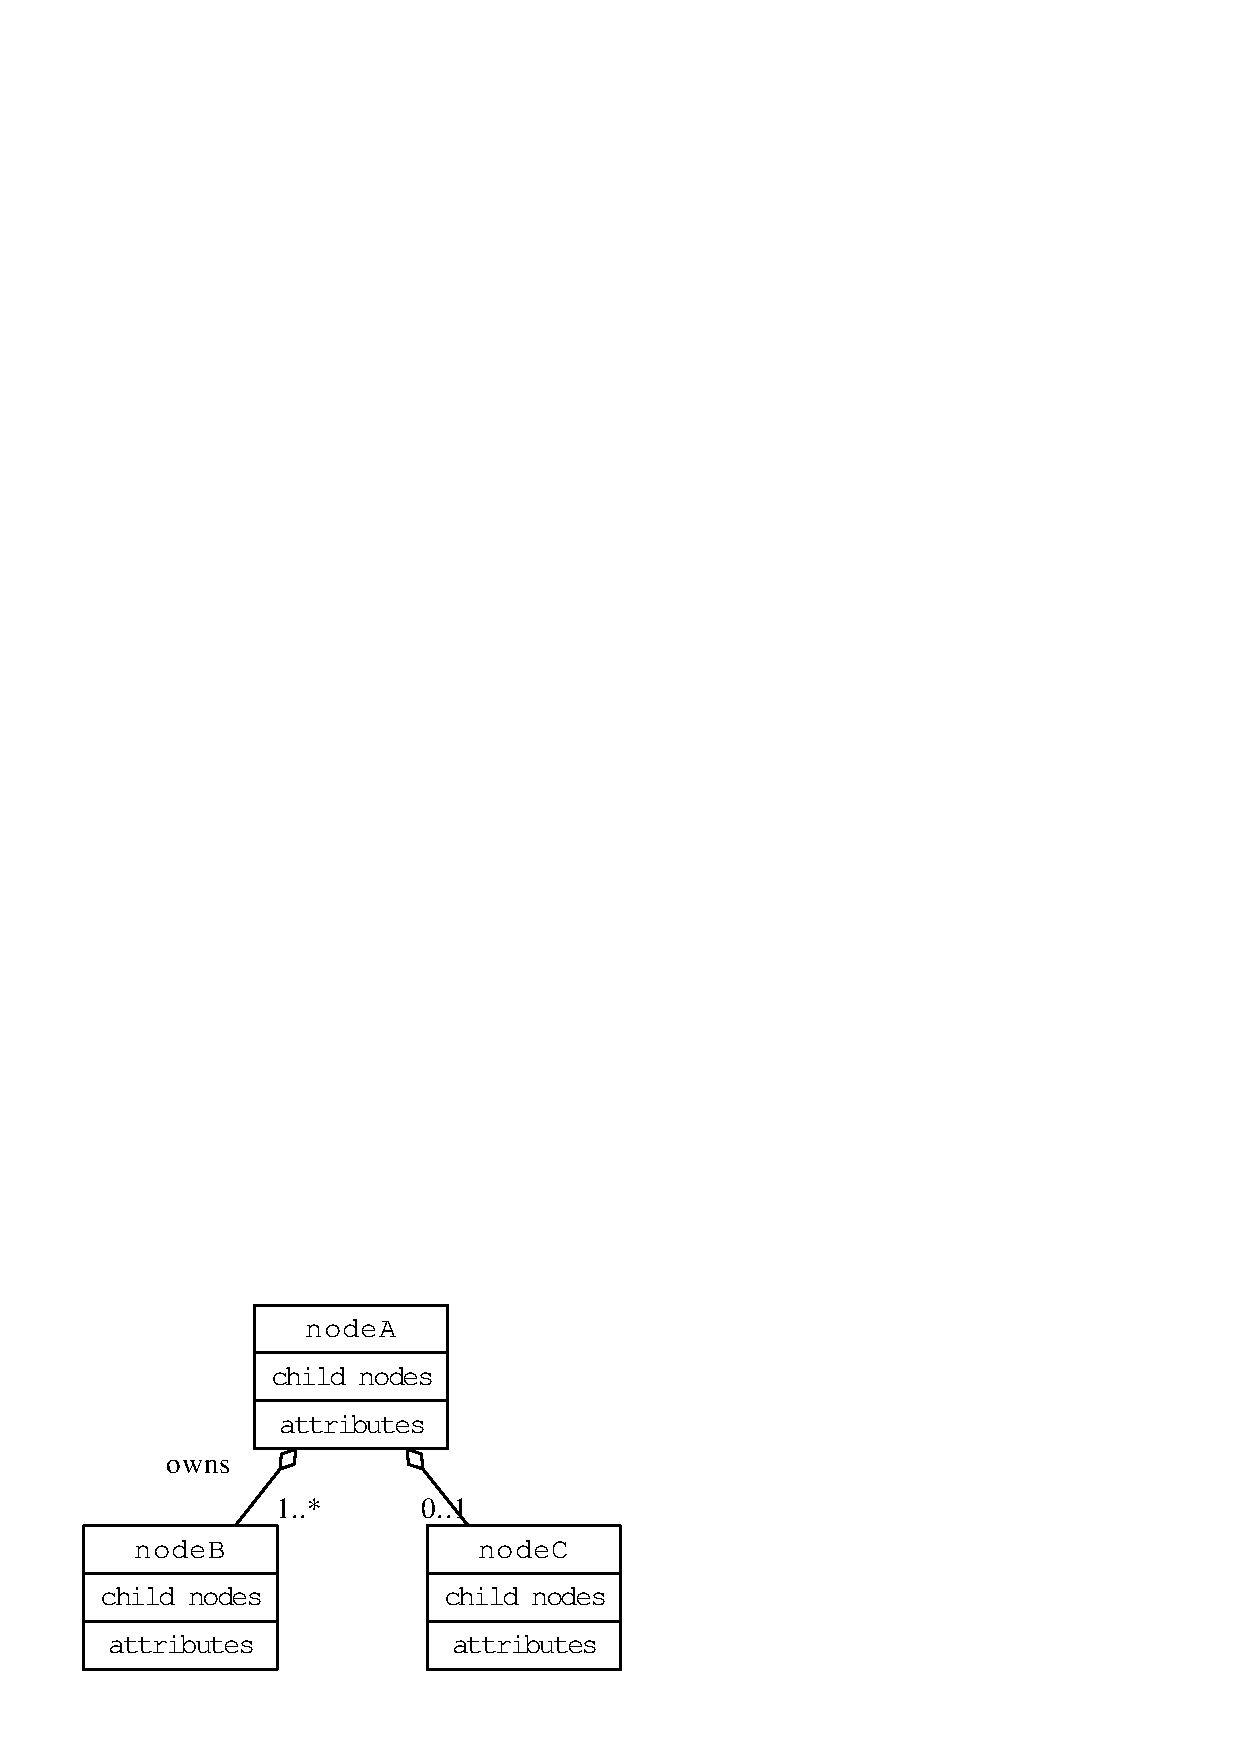
\includegraphics[width=0.5\textwidth,height=\textheight/2,keepaspectratio=true]{dot_xmlsymbols}
\caption{Graphical notations for a X\-M\-L node}
\end{DoxyImage}
 The opendiamond denotes the owndership\-: node\-A owns node\-B and node\-C. The multiplicity of child nodes is specificed at the child-\/node end.

Q\-M\-C\-P\-A\-C\-K uses D\-O\-M parser of {\tt libxml2} library. The entire input X\-M\-L file is parsed and stored in a tree which is processed recursively. Parsing a X\-M\-L file is similar to running a shell script. Each X\-M\-L element (node) is mapped to a factory or builder function to instantiate the main computational objects or to execute a class member function to initialize of the object which owns the node. The order of X\-M\-L nodes is critical to instantiate objects with proper ownerships and roles. All these features are exploited by the developers at the design stage of a particular class and algorithm in Q\-M\-C\-P\-A\-C\-K.

X\-M\-L files can be manipulated by standard editors and tools including web browsers. New features can be easily added without breaking the logical structure of the existing input files in X\-M\-L. Q\-M\-C\-P\-A\-C\-K requires a validating X\-M\-L but does not enforce correctness with a schema. This is mainly because Q\-M\-C\-P\-A\-C\-K is evolving quite rapidly and the input file is subject to change when new capabilities are added. A schema for the tested and accepted features is presented in this document and will be updated so that the new features can be utilized by the users as soon as they become available.\section{Reserved attributes and their implicit relationships}\label{a00004_attributeX}
These attributes are reserved to define the relationship between X\-M\-L nodes.


\begin{DoxyItemize}
\item {\ttfamily id} has to be unique in a given X\-M\-L file.
\item {\ttfamily name} is used as the name of an object. If {\ttfamily id} is not provided, {\ttfamily name} is used as the I\-D of the object.
\item {\ttfamily type} means the object or engine to be used at the run time.
\item {\ttfamily target} denotes the name (I\-D) of the quantum {\ttfamily particleset} (e.\-g., electrons).
\item {\ttfamily source} denotes the name (I\-D) of the source {\ttfamily particleset} (any fixed set of particles).
\end{DoxyItemize}

A X\-M\-L element has a well-\/defined scope. Child nodes inherit the property of a parent node. When a X\-M\-L node is referred by {\ttfamily ref}, {\ttfamily source} and {\ttfamily target}, the named X\-M\-L node has to be defined before using it.\section{simulation\-: Root element}\label{a00004_simX-ele}
{\ttfamily simulation} is the root element of the main input file and contains everything about a Q\-M\-C run. 
\begin{DoxyCode}
simulation = 
  children : project,
             (qmcsystem,particleset,wavefunction,hamiltonian,include)*,
             init?,
             loop?,
             qmc?
\end{DoxyCode}



\begin{DoxyImage}
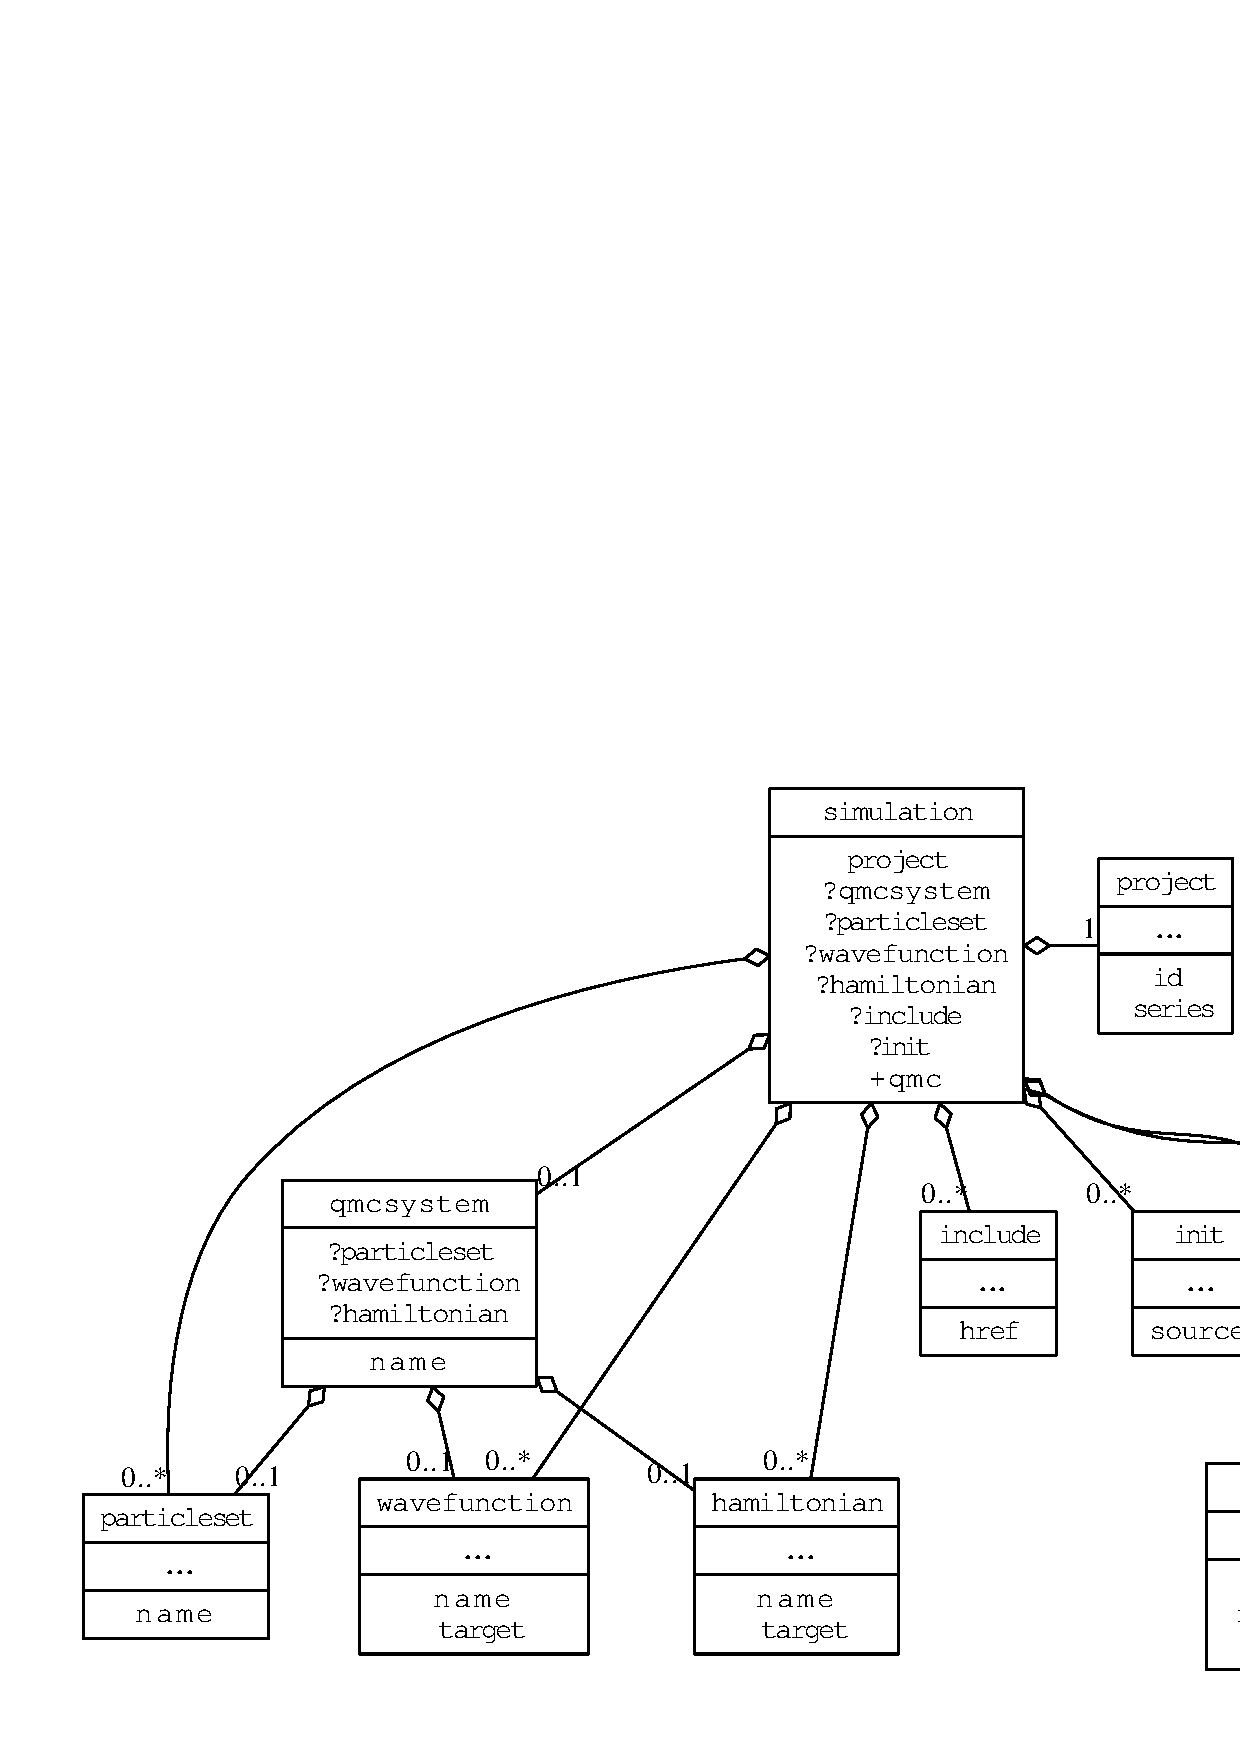
\includegraphics[width=\textwidth,height=\textheight/2,keepaspectratio=true]{dot_simulation}
\caption{simulation element}
\end{DoxyImage}
 \section{Generic X\-M\-L elements}\label{a00004_gen-xml}
These elements are used by other elements.\subsection{parameter}\label{a00004_parameterX}
This is a generic way to define a property of a X\-M\-L element and contains 
\begin{DoxyCode}
parameter = 
  children  : text \textcolor{keywordflow}{for} the value
  attribute : name
\end{DoxyCode}


For example, {\ttfamily parameter}s define how a V\-M\-C will be executed\-: 
\begin{DoxyCode}
<qmc method=\textcolor{stringliteral}{"vmc"}>
  <parameter name=\textcolor{stringliteral}{"timestep"}>0.5</parameter>
  <parameter name=\textcolor{stringliteral}{"blocks"}>10</parameter>
  <parameter name=\textcolor{stringliteral}{"steps"}>10</parameter>
  <parameter name=\textcolor{stringliteral}{"warmupsteps"}>10</parameter>
</qmc>
\end{DoxyCode}


Synopsis
\begin{DoxyItemize}
\item {\ttfamily parameter/@name} is the key of the parameter map in the application. The allowed {\ttfamily parameter}s and their usage are determined by their parent element.
\item Attribute {\ttfamily units} is reserved.
\end{DoxyItemize}

\begin{DoxyWarning}{Warning}
The type checking is handled by C++ {\ttfamily static\-\_\-cast$<$T$>$} and does not report nor abort the execution upon failure.
\end{DoxyWarning}
\subsection{include}\label{a00004_includeX}
{\ttfamily include} is used to include an external file\-: 
\begin{DoxyCode}
include = attribute : href
\end{DoxyCode}


The main input file can contain complete information about a Q\-M\-C simulation. However, it is often convenient to have multiple files to define different entities to manage multiple runs without needing to edit files and to automate the bulk of a workflow.

An example below includes three external files. Typically, conversion tools generate {\ttfamily ptcl.\-xml} and {\ttfamily wfs.\-xml}. The actual names may differ.


\begin{DoxyCode}
<simulation>
  <include href=\textcolor{stringliteral}{"ptcl.xml"}> <!-- define  ions and electrons -->
  <include href=\textcolor{stringliteral}{"wfs.xml"}> <!-- trial wavefunction -->
  <include href=\textcolor{stringliteral}{"ham.xml"}>  <!-- hamiltonian -->
  <!-- now \textcolor{keywordflow}{do} QMC -->

</simulation>
\end{DoxyCode}


Synopsis
\begin{DoxyItemize}
\item The included file has to be valid X\-M\-L with {\ttfamily qmcsystem} as its root element.
\item The order of {\ttfamily include} is strict and only one level of include is allowed, i.\-e., the external files cannot have any {\ttfamily include} element.
\end{DoxyItemize}

\begin{TabularC}{4}
\hline
\rowcolor{lightgray}{\bf name }&{\bf definition }&{\bf default }&{\bf comments}\\\cline{1-4}
href &Name of an external xml &node &A valid xml file \\\cline{1-4}
\end{TabularC}
\subsection{attrib}\label{a00004_attribX}
This is a generic way to define an attribute of a {\ttfamily particleset}, such as positions.


\begin{DoxyCode}
attrib = 
  children  : text \textcolor{keywordflow}{for} the value 
  attribute : name, datatype, size
\end{DoxyCode}


The data (text node) of each attrib corresponds to an array of various types. {\ttfamily attrib/@size} determines the size of the array and the allowed {\ttfamily attrib/@datatype}s are
\begin{DoxyItemize}
\item int\-Array \-: integers
\item real\-Array \-: reals
\item pos\-Array \-: D-\/dim vectors
\item string\-Array \-: strings
\end{DoxyItemize}\section{System elements}\label{a00004_systemX}
These elements are used to define a physical system, such as {\ttfamily particleset} for a set of particles and {\ttfamily wavefunction} for a trial wave function and must proceed any {\ttfamily qmc} or {\ttfamily loop} elements that define how the Q\-M\-C calculations are carried out.\subsection{qmcsystem}\label{a00004_qmcsystemX}
A {\ttfamily qmcsystem} defines a system for a Q\-M\-C simulation and contains 
\begin{DoxyCode}
qmcsystem = 
  children : (simulationcell,particleset,wavefunction,hamiltonian)*
\end{DoxyCode}
 It is also the root of an external X\-M\-L included by the main X\-M\-L file by {\ttfamily include/@href}


\begin{DoxyImage}
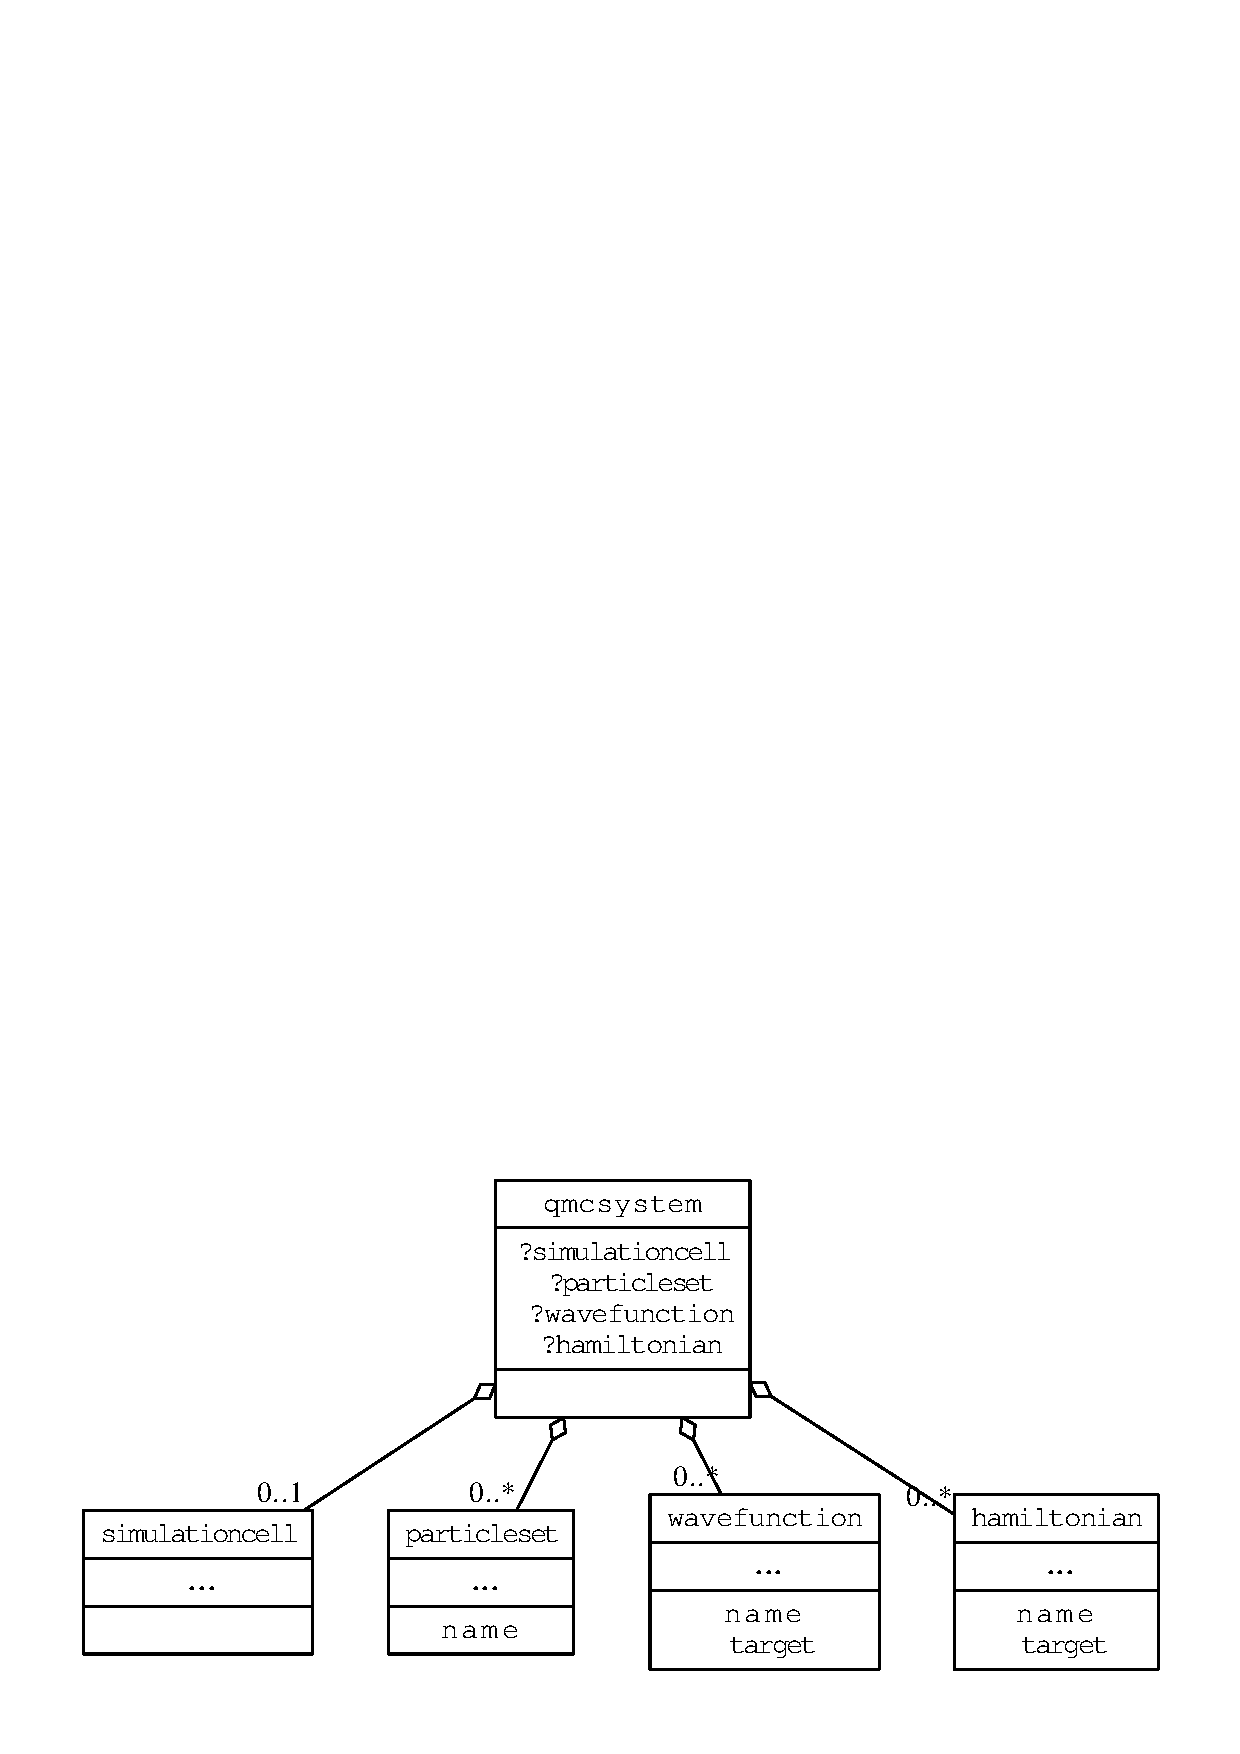
\includegraphics[width=0.75\textwidth,height=\textheight/2,keepaspectratio=true]{dot_qmcsys}
\caption{qmcsystem element}
\end{DoxyImage}
 Synopsis
\begin{DoxyItemize}
\item {\ttfamily qmcsystem} in the main input xml is not necessary but makes the input file more readable by grouping a number of elements to define a physical problem.
\item It defines a local scope. For example, {\ttfamily simulationcell} applies to all the {\ttfamily particleset}s in a {\ttfamily qmcsystem}
\end{DoxyItemize}\subsection{particleset}\label{a00004_particlesetX}
A {\ttfamily particleset} defines a set of particles and contains


\begin{DoxyCode}
particleset= 
  children  : group+, attrib*
  attribute : name, size, random, random\_source 
\end{DoxyCode}



\begin{DoxyImage}
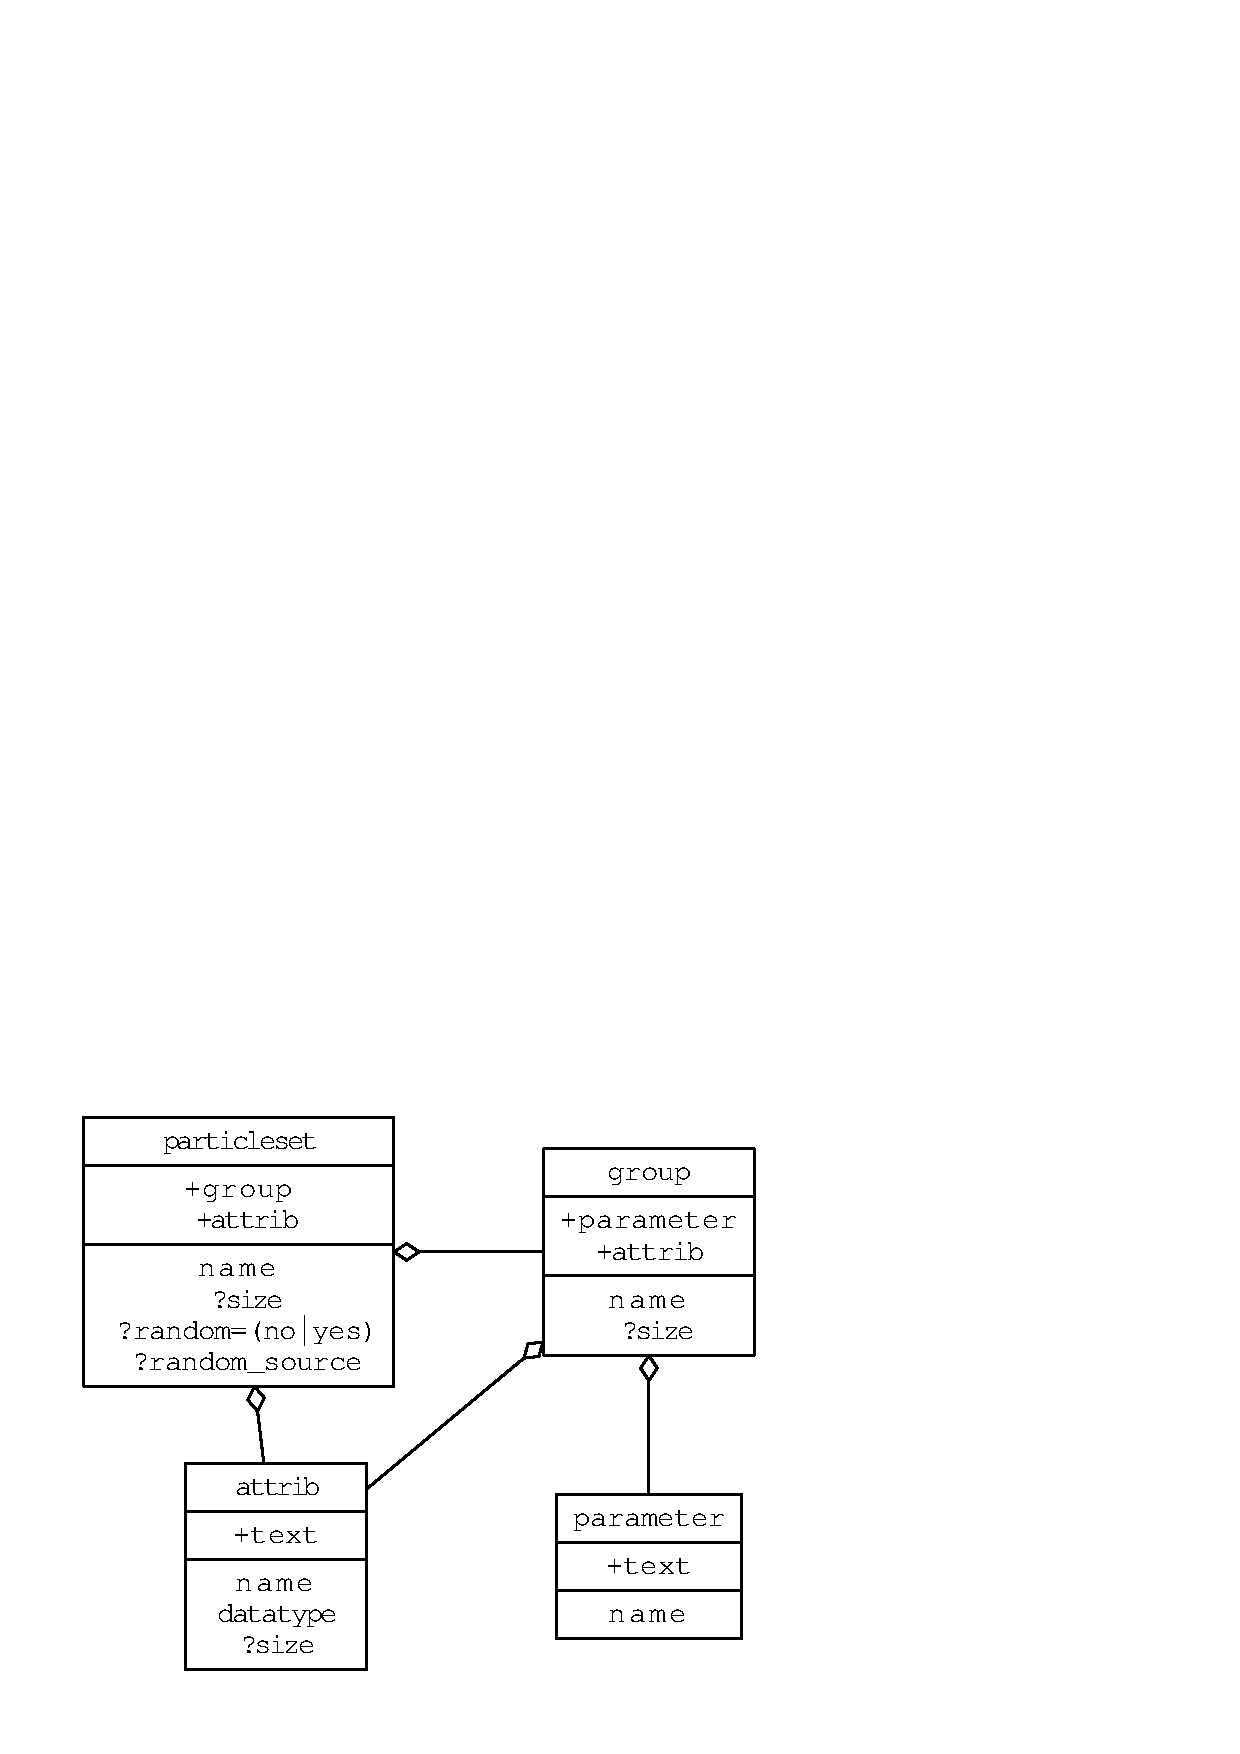
\includegraphics[width=0.5\textwidth,height=\textheight/2,keepaspectratio=true]{dot_particleset}
\caption{particleset element}
\end{DoxyImage}
 Attributes of {\ttfamily particleset} are

\begin{TabularC}{4}
\hline
\rowcolor{lightgray}{\bf name }&{\bf datatype }&{\bf default }&{\bf definition}\\\cline{1-4}
name &string &None &Name of this particle set. Referenced by other elements \\\cline{1-4}
size &integer &0 &Number of particles, when size is missing, {\ttfamily group/@size} is used \\\cline{1-4}
random &yes/no &no &Randomize the initial position. \\\cline{1-4}
random\-\_\-source &string &None &See the note on randomization of particle position \\\cline{1-4}
\end{TabularC}


If random==yes, the initial position of a {\ttfamily particleset} is randomonly assigned. The additional attribute {\ttfamily random\-\_\-source} can be provided to randomize the initial position with respect to a center {\ttfamily particleset}, typically an ionic system. The initialization attemps to use the {\ttfamily valence} charge of each ion set by either {\ttfamily particleset/group/param/@name} or by pseudopotentials. If {\ttfamily random\-\_\-source} is not given, positions are random values $[0,1)^D$ with respect to a simulationcell.

Synopsis
\begin{DoxyItemize}
\item It is seldom necessary for the users to prepare {\ttfamily particleset} from scratch. The conversion tools from other packages will generate {\ttfamily particleset} elements.
\item The H\-D\-F5 wavefunction file in E\-S-\/\-H\-D\-F format contains everything. It is possible to omit {\ttfamily particleset} See the section on E\-S-\/\-H\-D\-F.
\end{DoxyItemize}

The example below defines $H_2O$ with i) an ionic system called {\ttfamily particleset/@name='ion0'} and ii) an electronic system {\ttfamily particleset/@name='e'}. The positions of electrons are randomly assigned around the ions.


\begin{DoxyCode}
<qmcsystem>
  <particleset name=\textcolor{stringliteral}{"ion0"}>
    <group name=\textcolor{stringliteral}{"O"} size=\textcolor{stringliteral}{"1"}>
      <parameter name=\textcolor{stringliteral}{"charge"}>6</parameter>
      <parameter name=\textcolor{stringliteral}{"valence"}>4</parameter>
      <parameter name=\textcolor{stringliteral}{"atomicnumber"}>8</parameter>
      <attrib name=\textcolor{stringliteral}{"position"} datatype=\textcolor{stringliteral}{"posArray"}>
      0.0000000000e+00  0.0000000000e+00  0.0000000000e+00
      </attrib>
    </group>
    <group name=\textcolor{stringliteral}{"H"} size=\textcolor{stringliteral}{"2"}>
      <parameter name=\textcolor{stringliteral}{"charge"}>1</parameter>
      <parameter name=\textcolor{stringliteral}{"valence"}>1</parameter>
      <parameter name=\textcolor{stringliteral}{"atomicnumber"}>1</parameter>
      <attrib name=\textcolor{stringliteral}{"position"} datatype=\textcolor{stringliteral}{"posArray"}>
      0.0000000000e+00 -1.4304287043e+00  1.1071569627e+00
      0.0000000000e+00  1.4304287043e+00  1.1071569627e+00
      </attrib>
    </group>
  </particleset>
  <particleset name=\textcolor{stringliteral}{"e"} random=\textcolor{stringliteral}{"yes"} random\_source=\textcolor{stringliteral}{"ion0"}>
    <group name=\textcolor{stringliteral}{"u"} size=\textcolor{stringliteral}{"4"}>
      <parameter name=\textcolor{stringliteral}{"charge"}>-1</parameter>
    </group>
    <group name=\textcolor{stringliteral}{"d"} size=\textcolor{stringliteral}{"4"}>
      <parameter name=\textcolor{stringliteral}{"charge"}>-1</parameter>
    </group>
  </particleset>
</qmcsystem>
\end{DoxyCode}
\subsection{group}\label{a00004_groupX}
Defines a group of particles or species. 
\begin{DoxyCode}
group =
  children  : parameter+, attrib*
  attribute : name, size
\end{DoxyCode}


The properties of each group are defined by {\ttfamily parameter}. The parameters below are predefined in Q\-M\-C\-P\-A\-C\-K and their uses are restricted.

Attributes of {\ttfamily attrib}

\begin{TabularC}{4}
\hline
\rowcolor{lightgray}{\bf name }&{\bf datatype }&{\bf default }&{\bf definition}\\\cline{1-4}
charge &real &0 &Charge in atomic unit. q=-\/1 for the electrons \\\cline{1-4}
valence &real &0 &valence charge in A\-U \\\cline{1-4}
atomicnumber &integer &0 &Atomic number in the periodic table \\\cline{1-4}
\end{TabularC}


Synopsis
\begin{DoxyItemize}
\item Default {\ttfamily group/@size='0'}
\item When {\ttfamily group/@size} is provided, the {\ttfamily attrib}s within this group have the same size.
\end{DoxyItemize}\subsection{simulationcell}\label{a00004_simulationcellX}
A {\ttfamily simulationcell} defines the supercell of a Q\-M\-C simulation and contains 
\begin{DoxyCode}
simulationcell = children : parameter+
\end{DoxyCode}


As the name implies, {\ttfamily simulationcell} is only needed for bulk systems with periodic boundary conditions. One exception is when the single-\/particle orbitals ({\ttfamily S\-P\-O\-Set}) are represented by 3\-D tricubic bspline. Then, {\ttfamily simulationcell} should match the bounding box of the {\ttfamily S\-P\-O\-Set}.

{\ttfamily parameter}s provide the specific properties of a supercell as listed below.

\begin{TabularC}{4}
\hline
\rowcolor{lightgray}{\bf name }&{\bf definition }&{\bf default }&{\bf comments}\\\cline{1-4}
lattice &supercell vectors &$a(i,j)=\delta_{ij} 10^{10}$ &$a(i,j)$ denotes the i-\/th vector and the j-\/th component \\\cline{1-4}
scale &scaling factor to lattice &1.\-0 &Multiplied to {\ttfamily lattice} \\\cline{1-4}
bconds &boundary condition &p p p &Required For each lattice vector. p for Periodic and n for non-\/periodic \\\cline{1-4}
L\-R\-\_\-dim\-\_\-cutoff &cutoff radius &15 &Used for the optimized method (Natoli et al, J\-C\-P) for long-\/range potentials and Jastrow functions \\\cline{1-4}
rs &H\-E\-G density &1 &used to set the supercell for a homegenous electron gas. \\\cline{1-4}
\end{TabularC}


This is an example how to define a {\ttfamily simulationcell} and two {\ttfamily particleset}s. 
\begin{DoxyCode}
<qmcsystem>
  <simulationcell name=\textcolor{stringliteral}{"global"}>
    <!-- 3D Lattice 0x 0y 0z 1x 1y 1z 2x 2y 2z -->
    <parameter name=\textcolor{stringliteral}{"lattice"} units=\textcolor{stringliteral}{"bohr"}> 
    20.521733294552881    0.000000000000000    0.000000000000000
     0.000000000000000   20.521733294552881    0.000000000000000
     0.000000000000000    0.000000000000000   20.521733294552881
    </parameter>
    <!-- periodic boundary conditions -->
    <parameter name=\textcolor{stringliteral}{"bconds"}>p p p</parameter> 
    <parameter name=\textcolor{stringliteral}{"LR\_dim\_cutoff"}>15</parameter> 
  </simulationcell>
  <particleset name=\textcolor{stringliteral}{"ion0"}/> <!-- ionic system -->
  <particleset name=\textcolor{stringliteral}{"e"}/>    <!-- electronic system -->
</qmcsystem>
\end{DoxyCode}


Synopsis 
\begin{DoxyItemize}
\item When {\ttfamily simulationcell} is not provided, open boundary conditions are assumed. This is the default mode for the molecular systems. The wavefunction conversion tools for Quantum Chemistry codes using Gaussian-\/type orbitals do not insert {\ttfamily simulationcell} element.  
\item Specialized methods to evaluate the distance relationship between {\ttfamily particleset}s are selected based on the lattice type and boundary conditions. 


\item Particle moves outside of the supercell in the open direction(s) are rejected with bspline S\-P\-Os. For instance, the z coordinate of an electron is restricted to $[0,L_z)$ in a slab geomtry of Fig. Z\-Z\-Z. 
\end{DoxyItemize}\subsection{Restrictions for boundary conditions}\label{a00004_bcondsR}
For the electronic structure calculations in the P\-W basis, the gemoetric center of the ionic coordinates in the open-\/boundary directions has to be close to the center as illustrated in Fig. Z\-Z\-Z. It is because the values of the S\-P\-Os are not defined beyond the supercell. Since Q\-M\-C uses the values and the gradients of the S\-P\-Os which are normally represented by bsplines on a grid, it is important to apply strick convergence conditions on the vacuum region for the P\-W calculations to minimize the contributions from image cells. Not only the total energy should be converged with respect to the supercell, all the S\-P\-Os should decay to zero at the open boundaries.\subsection{hamiltonian}\label{a00004_hamiltonianX}
It defines a many-\/body Hamiltonian $\hat{H}=\sum_i \hat{h}$ for the target {\ttfamily particleset} to evaluate the local energy, \[ E_L({\bf R})=\frac{\hat{H}\Psi_T({\bf R})}{\Psi_T({\bf R})}. \]

{\bfseries R} denotes the configuration of the target {\ttfamily particleset} It contains 
\begin{DoxyCode}
hamiltonian = 
  children  : pairpot*, estimator*
  attribute : name, target, wavefunction
\end{DoxyCode}



\begin{DoxyImage}
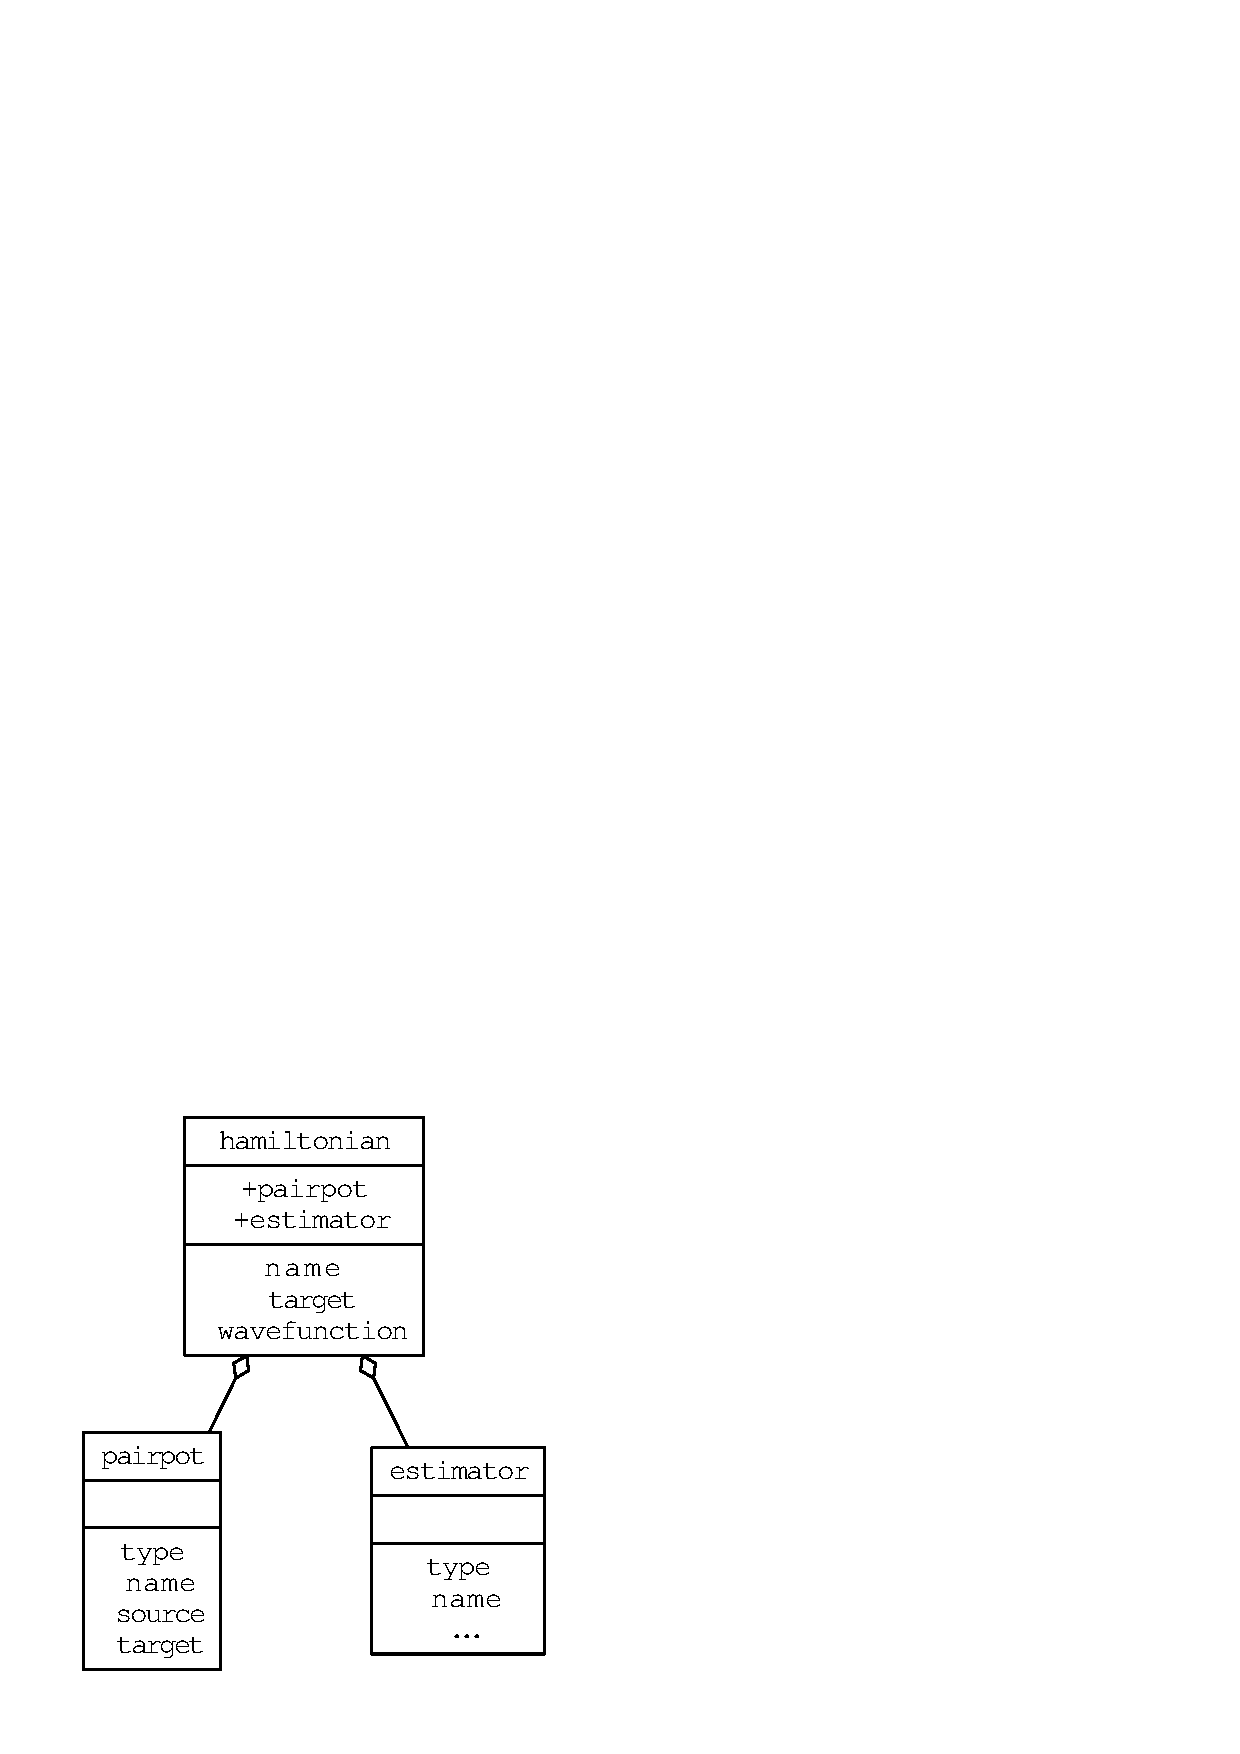
\includegraphics[width=0.5\textwidth,height=\textheight/2,keepaspectratio=true]{dot_hamiltonian}
\caption{hamiltonian element}
\end{DoxyImage}
 The attributes are \begin{TabularC}{4}
\hline
\rowcolor{lightgray}{\bf name }&{\bf definition }&{\bf default }&{\bf comments}\\\cline{1-4}
name &Name of this Hamiltonian &h0 &{\ttfamily hamiltonian/@name} is used when multiple {\ttfamily hamiltonian}s are used. \\\cline{1-4}
target &Target {\ttfamily particleset} &e &The default for quantum {\ttfamily particleset/@name=\char`\"{}e\char`\"{}} \\\cline{1-4}
wavefunction &Target {\ttfamily wavefunction} &psi0 &Non-\/local P\-P needs {\ttfamily wavefunction} \\\cline{1-4}
\end{TabularC}


Synopsis
\begin{DoxyItemize}
\item The children of {\ttfamily hamiltonian} are divided into
\begin{DoxyItemize}
\item Physical operator, $\hat{h}$, whose value is added to the local energy.
\item Estimators for an operator $O = \hat O\Psi_T/\Psi_T$
\end{DoxyItemize}
\item The kinetic operator is automatically added to the total $\hat{H}$.
\item {\bfseries Advanced} It is possible to overwrite the kinetic operator with a specialized kinetic operator.
\end{DoxyItemize}

A typical {\ttfamily hamiltonian} with pseudopotentials is 
\begin{DoxyCode}
<hamiltonian name=\textcolor{stringliteral}{"h0"} type=\textcolor{stringliteral}{"generic"} target=\textcolor{stringliteral}{"e"}>
 <pairpot name=\textcolor{stringliteral}{"ElecElec"} type=\textcolor{stringliteral}{"coulomb"} source=\textcolor{stringliteral}{"e"} target=\textcolor{stringliteral}{"e"}/>
 <pairpot name=\textcolor{stringliteral}{"IonIon"} type=\textcolor{stringliteral}{"coulomb"} source=\textcolor{stringliteral}{"ion0"} target=\textcolor{stringliteral}{"ion0"}/>
 <pairpot name=\textcolor{stringliteral}{"PseudoPot"} type=\textcolor{stringliteral}{"pseudo"} source=\textcolor{stringliteral}{"ion0"} 
          wavefunction=\textcolor{stringliteral}{"psi0"} format=\textcolor{stringliteral}{"xml"}>
   <pseudo elementType=\textcolor{stringliteral}{"C"} href=\textcolor{stringliteral}{"C.BFD.xml"} format=\textcolor{stringliteral}{"xml"}/>
 </pairpot>
 <!-- finite-size correction -->
 <estimator name=\textcolor{stringliteral}{"KEcorr"} type=\textcolor{stringliteral}{"chiesa"} source=\textcolor{stringliteral}{"e"} psi=\textcolor{stringliteral}{"psi0"}/> 
</hamiltonian>
\end{DoxyCode}
\subsubsection{pairpot}\label{a00004_pairpotX}
It defines a pair potential and contains 
\begin{DoxyCode}
pairpot = attribute : name, type, source, target, wavefunction
\end{DoxyCode}


The names of {\ttfamily source}, {\ttfamily target} and {\ttfamily wavefunction} must be those of the existing objects. {\ttfamily wavefunction} is necessary with non-\/local pseudopotentials.

The attributes are \begin{TabularC}{4}
\hline
\rowcolor{lightgray}{\bf name }&{\bf definition }&{\bf default }&{\bf comments}\\\cline{1-4}
type &Potential type &None &Choose\-: coulomb, pseudo \\\cline{1-4}
source &Source {\ttfamily particleset} &None &Required \\\cline{1-4}
target &Target {\ttfamily particleset} &{\ttfamily target} of the parent element &Optional, inherited from {\ttfamily hamiltonian} \\\cline{1-4}
\end{TabularC}


Synopsis
\begin{DoxyItemize}
\item Any operator expressed as $ V=\sum_{i}^{source}\sum_{j}^{target} \phi({\bf r}_j,{\bf r}_i)$ is a candidate of {\ttfamily pairopot}, where each $\sum$ is over a {\ttfamily particleset}.
\item {\ttfamily pairpot/@type='coulomb'} is reserved for Coulomb potential. See section coulombsec.
\item {\ttfamily pairpot/@type='pseudo'} is reserved for pseudo potential. See section pseudosec.
\end{DoxyItemize}\subsection{wavefunction}\label{a00004_wfsX}
It defines a trial wavefunction \[\Psi_T=\prod_i \psi_i\] where $\psi_i$ is a many-\/body wavefunction component, e.\-g. a Slater-\/\-Jastrow orbital is \[\Psi_T = e^{J} \sum_k^{M} C_k D_{k}^{\uparrow}(\phi)D_k^{\downarrow}(\phi).\] Here, $\{\phi\}$ denotes a set of single-\/particle orbitals ({\ttfamily S\-P\-Os}). It contains 
\begin{DoxyCode}
wavefunction = 
  chidren : jastrow*, determinantset
  attribute : name, target
\end{DoxyCode}



\begin{DoxyImage}
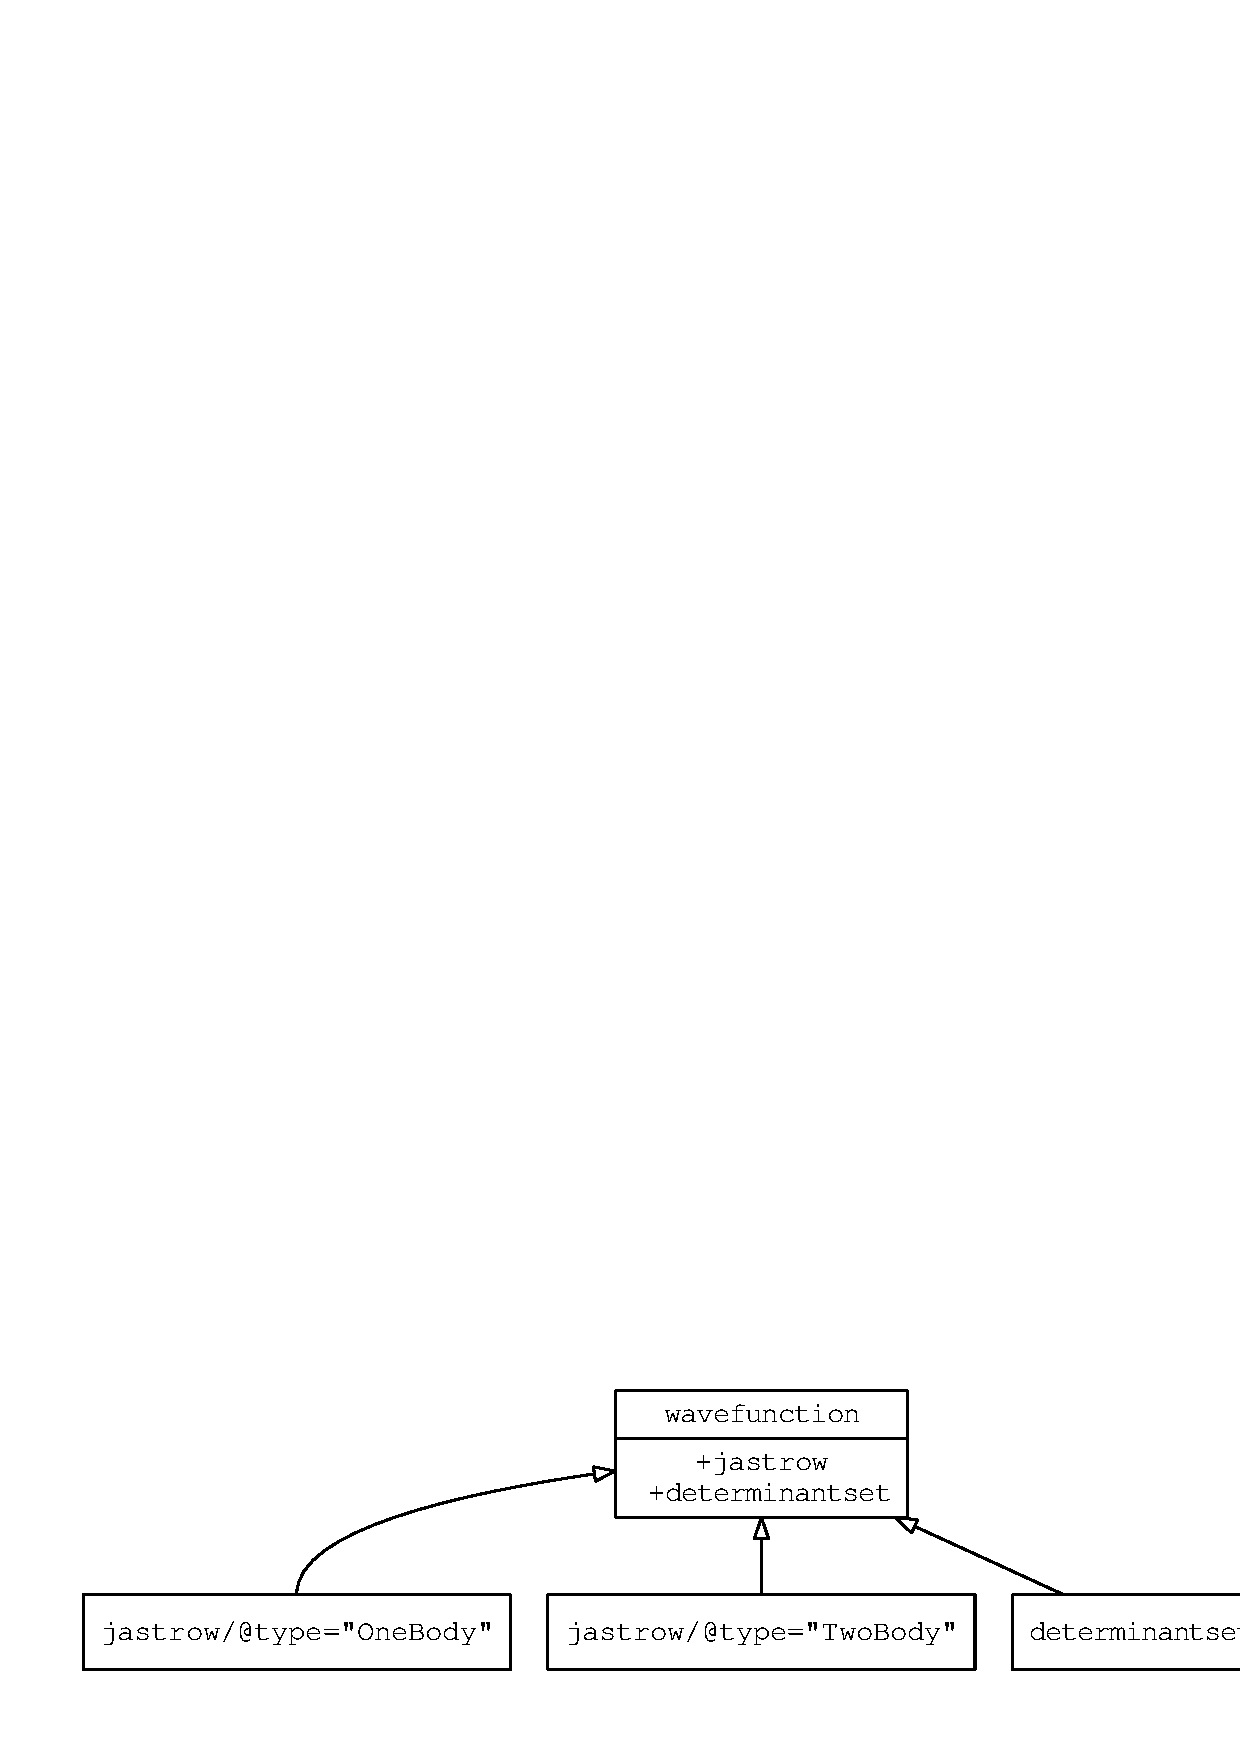
\includegraphics[width=\textwidth,height=\textheight/2,keepaspectratio=true]{dot_wfs}
\caption{wavefunction element}
\end{DoxyImage}
 The attributes are \begin{TabularC}{4}
\hline
\rowcolor{lightgray}{\bf name }&{\bf definition }&{\bf default }&{\bf comments}\\\cline{1-4}
name &Name of this wavefunction &psi0 &{\ttfamily wavefunction/@name} is used when multiple {\ttfamily wavefunction}s are used. \\\cline{1-4}
target &Target {\ttfamily particleset} &e &The default for quantum {\ttfamily particleset/@name=\char`\"{}e\char`\"{}} \\\cline{1-4}
\end{TabularC}


{\ttfamily wavefunction} is the most important element in Q\-M\-C calculations. Except for very simple toy problems, it is seldom possible to prepare a {\ttfamily wavefunction} from scratch. Also, it is highly propblem and theory depdenent and changing constantly.\subsubsection{jastrow}\label{a00004_jastrowX}

\begin{DoxyCode}
jastrow = attribute : name, type, \textcolor{keyword}{function}, source
\end{DoxyCode}


The attributes are \begin{TabularC}{4}
\hline
\rowcolor{lightgray}{\bf name }&{\bf definition }&{\bf default }&{\bf comments}\\\cline{1-4}
name &Name of this Jastrow &None &Unique value in an input \\\cline{1-4}
type &Type of this Jastrow &None &One\-Body, Two\-Body, Three\-Body \\\cline{1-4}
function &Scaling functor of this Jastrow &None &Bspline, pade \\\cline{1-4}
source &source {\ttfamily particleset} &None &Any {\ttfamily particleset} that can provide the centers. \\\cline{1-4}
\end{TabularC}


\label{a00004_j2def}%
Two-\/\-Body Jastrow

\[J2=\sum_i^{e}\sum_{j>i}^{e} u_{ab}(|{\bf r}_i-{\bf r}_j|)\]

Here, {\itshape a} and {\itshape b} denote u(p) electrons or d(own) electrons. The use of u for up electrons and d for down electrons are generally adopted by the users.


\begin{DoxyItemize}
\item The scale function $u(r)$ is defined for species pairs, uu, ud.  
\item There is no need to define, du and dd, since uu==dd and ud==du. 
\item cusp condition is computed internally based on the charge of the quantum particles. 
\item The type of scaling functions of this jastrow is ginve by {\ttfamily jastrow/@function}. The example selects {\ttfamily Bspline} (1\-D tricubic spline function on a linear grid).  
\end{DoxyItemize}

These are common use cases. 
\begin{DoxyItemize}
\item Two-\/body Jastrow with {\ttfamily Bspline} functor 
\begin{DoxyCode}
<jastrow name=\textcolor{stringliteral}{"J2"} type=\textcolor{stringliteral}{"Two-Body"} \textcolor{keyword}{function}=\textcolor{stringliteral}{"Bspline"} source=\textcolor{stringliteral}{"ion0"} spin=\textcolor{stringliteral}{"yes"}>
  <correlation speciesA=\textcolor{stringliteral}{"u"} speciesB=\textcolor{stringliteral}{"u"} size=\textcolor{stringliteral}{"7"} rcut=\textcolor{stringliteral}{"6"}>
    <coefficients \textcolor{keywordtype}{id}=\textcolor{stringliteral}{"uu"} type=\textcolor{stringliteral}{"Array"}> 
    0.0 0.0 0.0 0.0 0.0 0.0 0.0
    </coefficients>
  </correlation>
  <correlation speciesA=\textcolor{stringliteral}{"u"} speciesB=\textcolor{stringliteral}{"d"} size=\textcolor{stringliteral}{"7"} rcut=\textcolor{stringliteral}{"6"}>
    <coefficients \textcolor{keywordtype}{id}=\textcolor{stringliteral}{"ud"} type=\textcolor{stringliteral}{"Array"}> 
    0.0 0.0 0.0 0.0 0.0 0.0 0.0
    </coefficients>
  </correlation>
</jastrow>
\end{DoxyCode}
  
\end{DoxyItemize}

\label{a00004_j1def}%
One-\/\-Body Jastrow

\[J1=\sum_I^{ion0}\sum_i^{e} u_{ab}(|{\bf r}_i-{\bf R}_I|)\]


\begin{DoxyItemize}
\item {\ttfamily jastrow/@source} is the source {\ttfamily particleset}, typically an ionic system. 
\item The scale function $u_{ab}(r)$ is can be spin-\/independent when {\itshape b} applies to both spins or spin-\/dependent.  
\item The type of scaling functions of this jastrow is ginve by {\ttfamily jastrow/@function}. The example selects {\ttfamily Bspline} (1\-D tricubic spline function on a linear grid).  
\end{DoxyItemize}

These are common use cases. 
\begin{DoxyItemize}
\item Spin-\/independent one-\/body Jastrow with {\ttfamily Bspline} functor 
\begin{DoxyCode}
<jastrow name=\textcolor{stringliteral}{"J1"} type=\textcolor{stringliteral}{"One-Body"} \textcolor{keyword}{function}=\textcolor{stringliteral}{"Bspline"} source=\textcolor{stringliteral}{"ion0"}>
  <correlation elementType=\textcolor{stringliteral}{"C"} size=\textcolor{stringliteral}{"7"} rcut=\textcolor{stringliteral}{"6"}>
    <coefficients \textcolor{keywordtype}{id}=\textcolor{stringliteral}{"eC"} type=\textcolor{stringliteral}{"Array"}> 
    0.0 0.0 0.0 0.0 0.0 0.0 0.0
    </coefficients>
  </correlation>
</jastrow>
\end{DoxyCode}
  
\item Spin-\/dependent one-\/body Jastrow with {\ttfamily Bspline} functor 
\begin{DoxyCode}
<jastrow name=\textcolor{stringliteral}{"J1"} type=\textcolor{stringliteral}{"One-Body"} \textcolor{keyword}{function}=\textcolor{stringliteral}{"Bspline"} source=\textcolor{stringliteral}{"ion0"} spin=\textcolor{stringliteral}{"yes"}>
  <correlation speciesA=\textcolor{stringliteral}{"C"} speciesB=\textcolor{stringliteral}{"u"} size=\textcolor{stringliteral}{"7"} rcut=\textcolor{stringliteral}{"6"}>
    <coefficients \textcolor{keywordtype}{id}=\textcolor{stringliteral}{"eCu"} type=\textcolor{stringliteral}{"Array"}> 
    0.0 0.0 0.0 0.0 0.0 0.0 0.0
    </coefficients>
  </correlation>
  <correlation speciesA=\textcolor{stringliteral}{"C"} speciesB=\textcolor{stringliteral}{"d"} size=\textcolor{stringliteral}{"7"} rcut=\textcolor{stringliteral}{"6"}>
    <coefficients \textcolor{keywordtype}{id}=\textcolor{stringliteral}{"eCd"} type=\textcolor{stringliteral}{"Array"}> 
    0.0 0.0 0.0 0.0 0.0 0.0 0.0
    </coefficients>
  </correlation>
</jastrow>
\end{DoxyCode}
  
\end{DoxyItemize}

\begin{DoxyNote}{Note}
Both {\ttfamily correlation@element\-Type} and {\ttfamily correlation@species\-A} are accepted.
\end{DoxyNote}
\section{Execution of Q\-M\-C methods}\label{a00004_actionX}
\subsection{Q\-M\-C element}\label{a00004_qmcX}
It defines a Q\-M\-C run using various Q\-M\-C methods, e.\-g., variational Monte Carlo (vmc) or diffusion Monte Carlo (dmc). Any number of {\ttfamily qmc} can be given in an input file and each section is executed sequentially. 
\begin{DoxyCode}
qmc = 
  children  : parameter+ 
  attribute : name, target
\end{DoxyCode}
\subsection{Loop element}\label{a00004_loopX}
It defines a loop for the execution of executes the included {\ttfamily qmc} sections and contains 
\begin{DoxyCode}
loop = 
  children : qmc+
  attribute : max
\end{DoxyCode}
 
